% Chapter Template

\chapter{Dataset and Exploratory Analysis} % Main chapter title

\label{c3} % Change X to a consecutive number; for referencing this chapter elsewhere, use \ref{ChapterX}

%----------------------------------------------------------------------------------------
%	SECTION 1
%----------------------------------------------------------------------------------------
\section{Dataset and Exploratory Analysis}
 
\textbf({Exploratory Data Analysis(EDA)}): Dataset is taken from Physionet ATM. The PTB Diagnostic ECG Database \href{https://physionet.org/content/ptbdb/1.0.0}{(https://physionet.org/content/ptbdb/1.0.0)} consist of ECG reports of 294 subjects,  which includes healthy subjects as well as patients with various heart disease conditions. All datasets contain 10000 samples each. Data points are distributed in a cycle of 10 seconds each. Sampling rate is set to 1000. Single lead ECG data (lead-{II}) of five patients has been taken since PTB diagnostic ECG database is very large database with 290 subjects and it was not possible to study all individually hence we took five records with different distributions. Since majority among the researches evaluated the effectiveness of computer-aided methods on (lead-II) ECG,  which is taken in previous studies \cite{liu2021deep}. This is how they look Figure  \ref{Fig:1}. Here (P1, P2, P3, P4 and P5) are patient's recorded ECG :
\begin{figure*}[ht!]
    \centering
     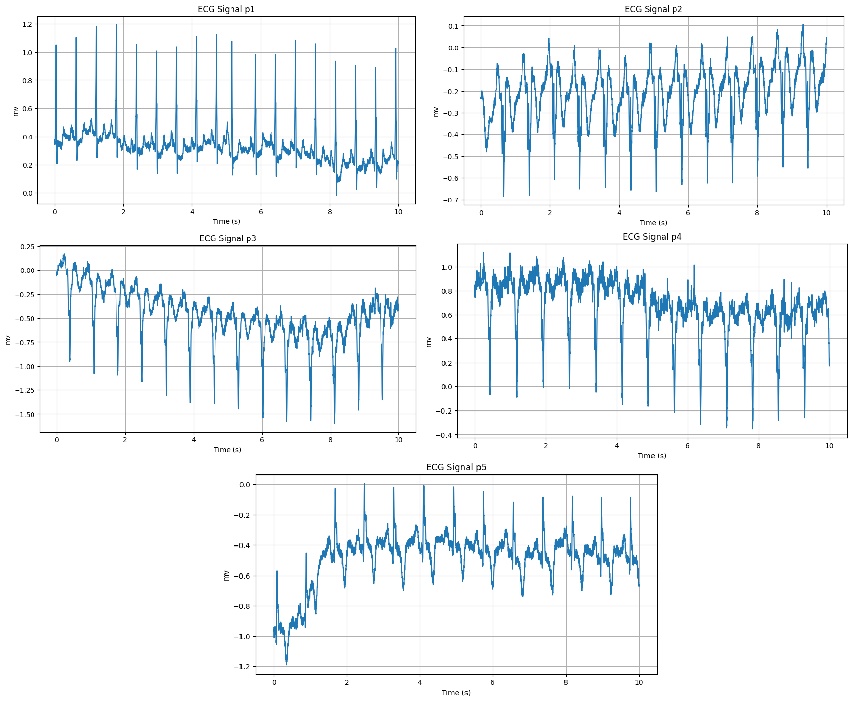
\includegraphics[scale=1]{edadrawio.pdf}
     \caption{Patient's(P1,  P2,  P3,  P4 and P5) ECG Plot}
     \label{Fig:1}
   \end{figure*}
\begin{figure*}[h!]
  \centering
   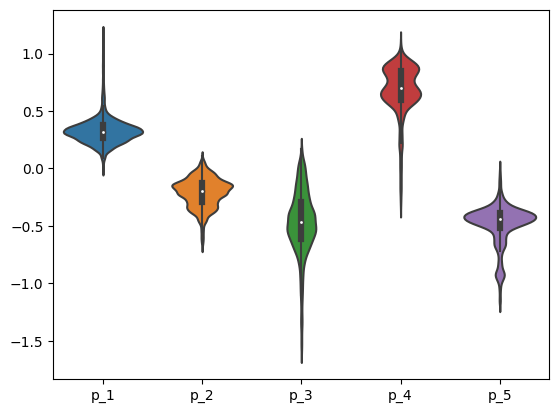
\includegraphics[scale=.5]{violin_plot_5_patients.png}
  \caption{Dataset distribution using violin plot}
   \label{Fig:2}
\end{figure*}

 
   \begin{figure*}[h!]
    \centering
     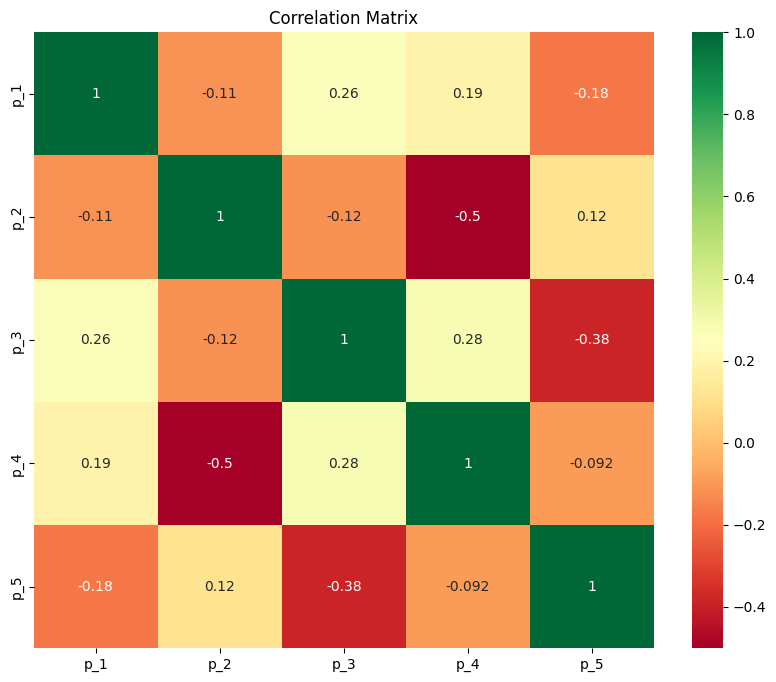
\includegraphics[scale=.42]{correlation_matrix_5_patients.png}
     \caption{Dataset's correlation matrix} 
     \label{Fig:3}
    \end{figure*} 

   \begin{figure*}[h!]
    \centering
     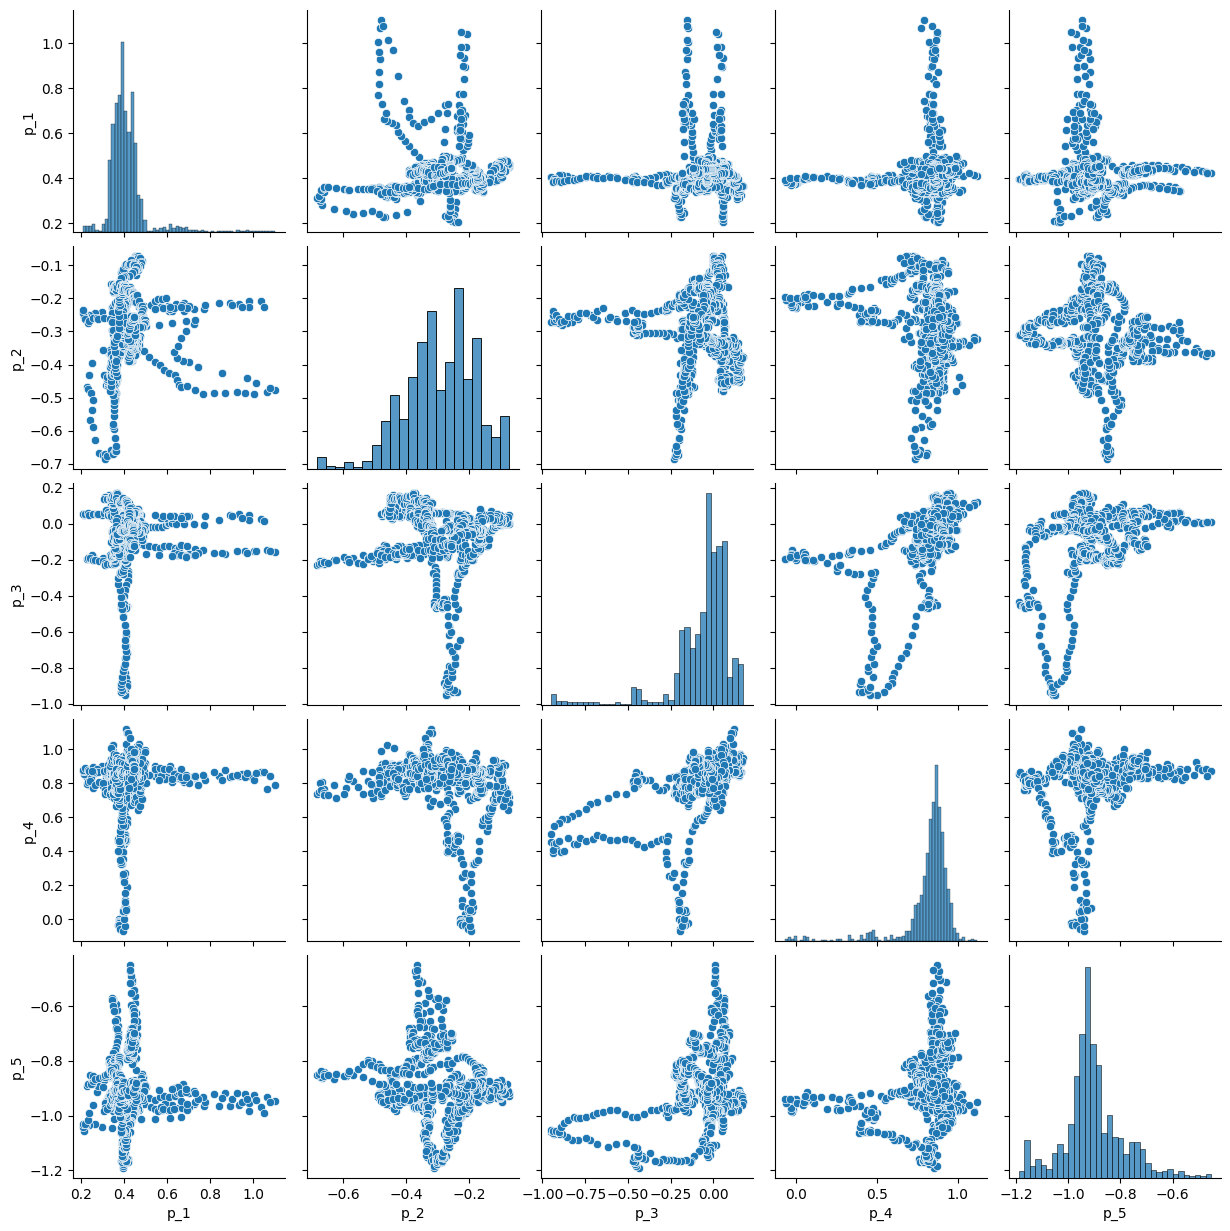
\includegraphics[scale=.52]{pair_plot.png}
     \caption{Patient's dataset distribution pair-plot}
    \label{Fig:4}
   \end{figure*}
  

 
 The plot has been drawn to look into distribution of our dataset With violin plot Figure  \ref{Fig:2} it can be understood whether the values are clustered around the median. Additionally,  it can be understood if the dataset values exhibit excessive clustering with an absence of values in the middle range. The Heatmap Figure  \ref{Fig:3} is representing correlation between the chosen datasets,  as it can be seen datasets with high collinearity are selected for studies. With pairplot Figure  \ref{Fig:4} pairwise relationship between datasets can be seen since it plots multiple pairwise bivariate distributions. The diagonal plots are univariate plots, and they show the relationship for the (n,  2) variable combination in a Dataframe as a matrix of plots.
Also  For time series analysis and dataset understanding,  statistical measures are used in conjunction with exploratory data analysis.
 


